\documentclass{article}
\usepackage{graphicx} %package to manage images
\usepackage[utf8]{inputenc}
\usepackage[a4paper, total={6in, 8in}]{geometry}
\usepackage{xurl}
\usepackage{hyperref}
\usepackage{float}
\title{Relatório 21 \\ Permutation test}
\author{Pedro A. S. O. Neto}
\date{Março, 2023}

\begin{document}

\maketitle

\section{Justificativa}

Após o processamento de dados e a aplicação de todos os filtros (descritos no Report 20), o $N$ de TEA = 15, e não TEA = 425.
Como forma de testar algumas estatísticas (i.e, proporção de fixações e números de alternâncias), decidimos utilizar um teste de permutação.

O procedimento estatístico é o seguinte:
\begin{itemize}
  \item Separa-se os participantes TEA de TD.
  \item Coleta-se um sub-sample da amostra total de participantes TD. O tamanho do sample é igual ao numero de participantes TEA (neste caso, 15).
  \item Computa-se a estatística de interesse para esse sample.
  \item Repete-se este processo N vezes, com reposição dos participantes retirados em cada sub-sample (o mesmo participante pode ser sampleado mais de uma vez).
\end{itemize}

Ao final deste processo, temos uma distribuição de sample da estatística de interesse. Então olhamos novamente para as estatísticas do sample de TEA, e computamos a probabilidade deste sample ter vindo da mesma população que os TD ($p-value$).

\section{Resultados}

\subsection{pValues - Proporções}

  \begin{table}[ht]
  \centering
  \begin{tabular}{rllrr}
    \hline
   & condition & variable & pValuesHigher & pValuesLower \\ 
    \hline
  1 & RJA & distractorProportion & 0.04 & 0.96 \\ 
    2 & RJA & fundoProportion & 0.01 & 0.99 \\ 
    3 & RJA & targetProportion & 1.00 & 0.00 \\ 
    4 & RJA & rostoProportion & 0.86 & 0.14 \\ 
    5 & IJA & distractorProportion & 0.15 & 0.85 \\ 
    6 & IJA & fundoProportion & 0.02 & 0.98 \\ 
    7 & IJA & targetProportion & 0.79 & 0.21 \\ 
    8 & IJA & rostoProportion & 0.73 & 0.27 \\ 
     \hline
  \end{tabular}
  \end{table}

\subsection{pValues - Alternâncias}

\begin{table}[ht]
\centering
\begin{tabular}{rllrr}
  \hline
 & condition & variable & pValuesHigher & pValuesLower \\ 
  \hline
1 & RJA & targetRosto & 0.98 & 0.02 \\ 
  2 & RJA & rostoTarget & 1.00 & 0.00 \\ 
  3 & RJA & distractorRosto & 0.97 & 0.03 \\ 
  4 & RJA & rostoDistractor & 0.94 & 0.07 \\ 
  5 & IJA & targetRosto & 0.94 & 0.06 \\ 
  6 & IJA & rostoTarget & 0.93 & 0.07 \\ 
  7 & IJA & distractorRosto & 0.46 & 0.54 \\ 
  8 & IJA & rostoDistractor & 0.68 & 0.32 \\ 
   \hline
\end{tabular}
\end{table}

\subsection{Proporção}

\begin{figure}[H]
  \caption{Média de tempo proporcional que participantes passam olhando para determinados pontos da tela. Linha pontilhada azul indica o sample de participantes com TEA.}
  \noindent\makebox[\textwidth]{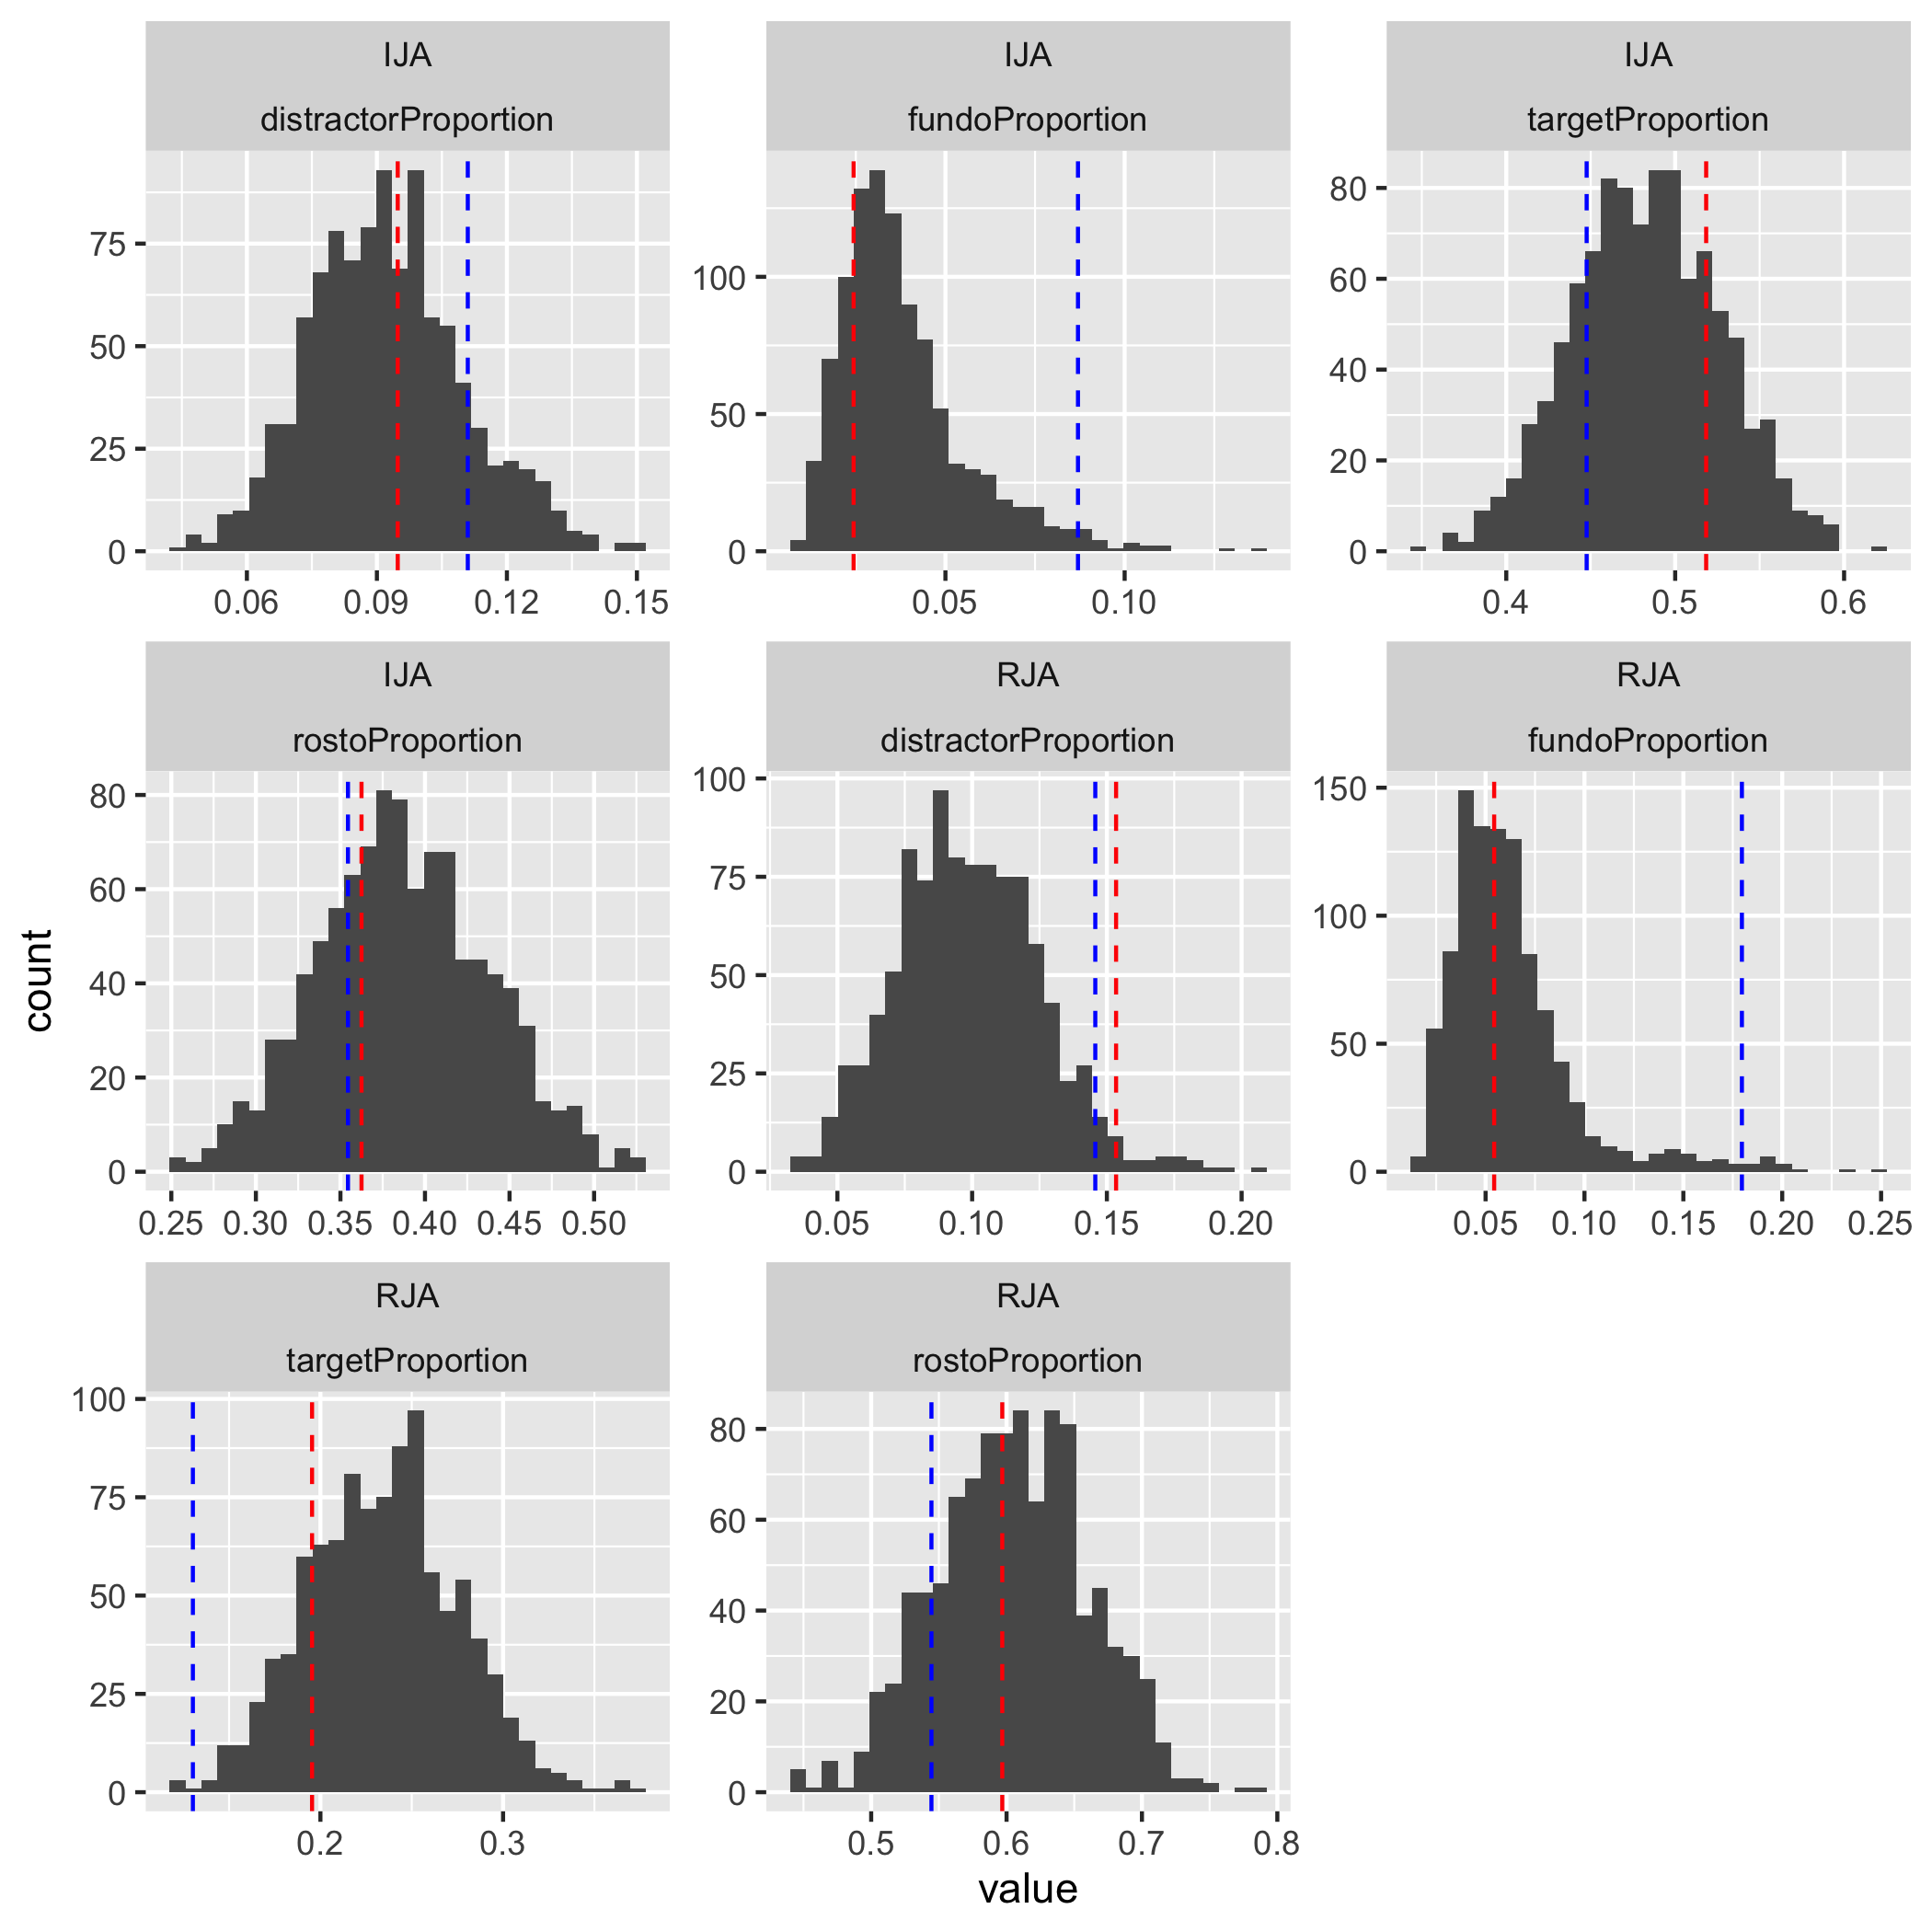
\includegraphics[scale=0.2]{./proportionsTEAandNonTD.png}}
  \centering
\end{figure}

\subsection{Alternância}

\begin{figure}[H]
  \caption{Média de alternâncias realizadas entre diferentes regiões da tela. Linha pontilhada azul indica o sample de participantes com TEA.}
  \noindent\makebox[\textwidth]{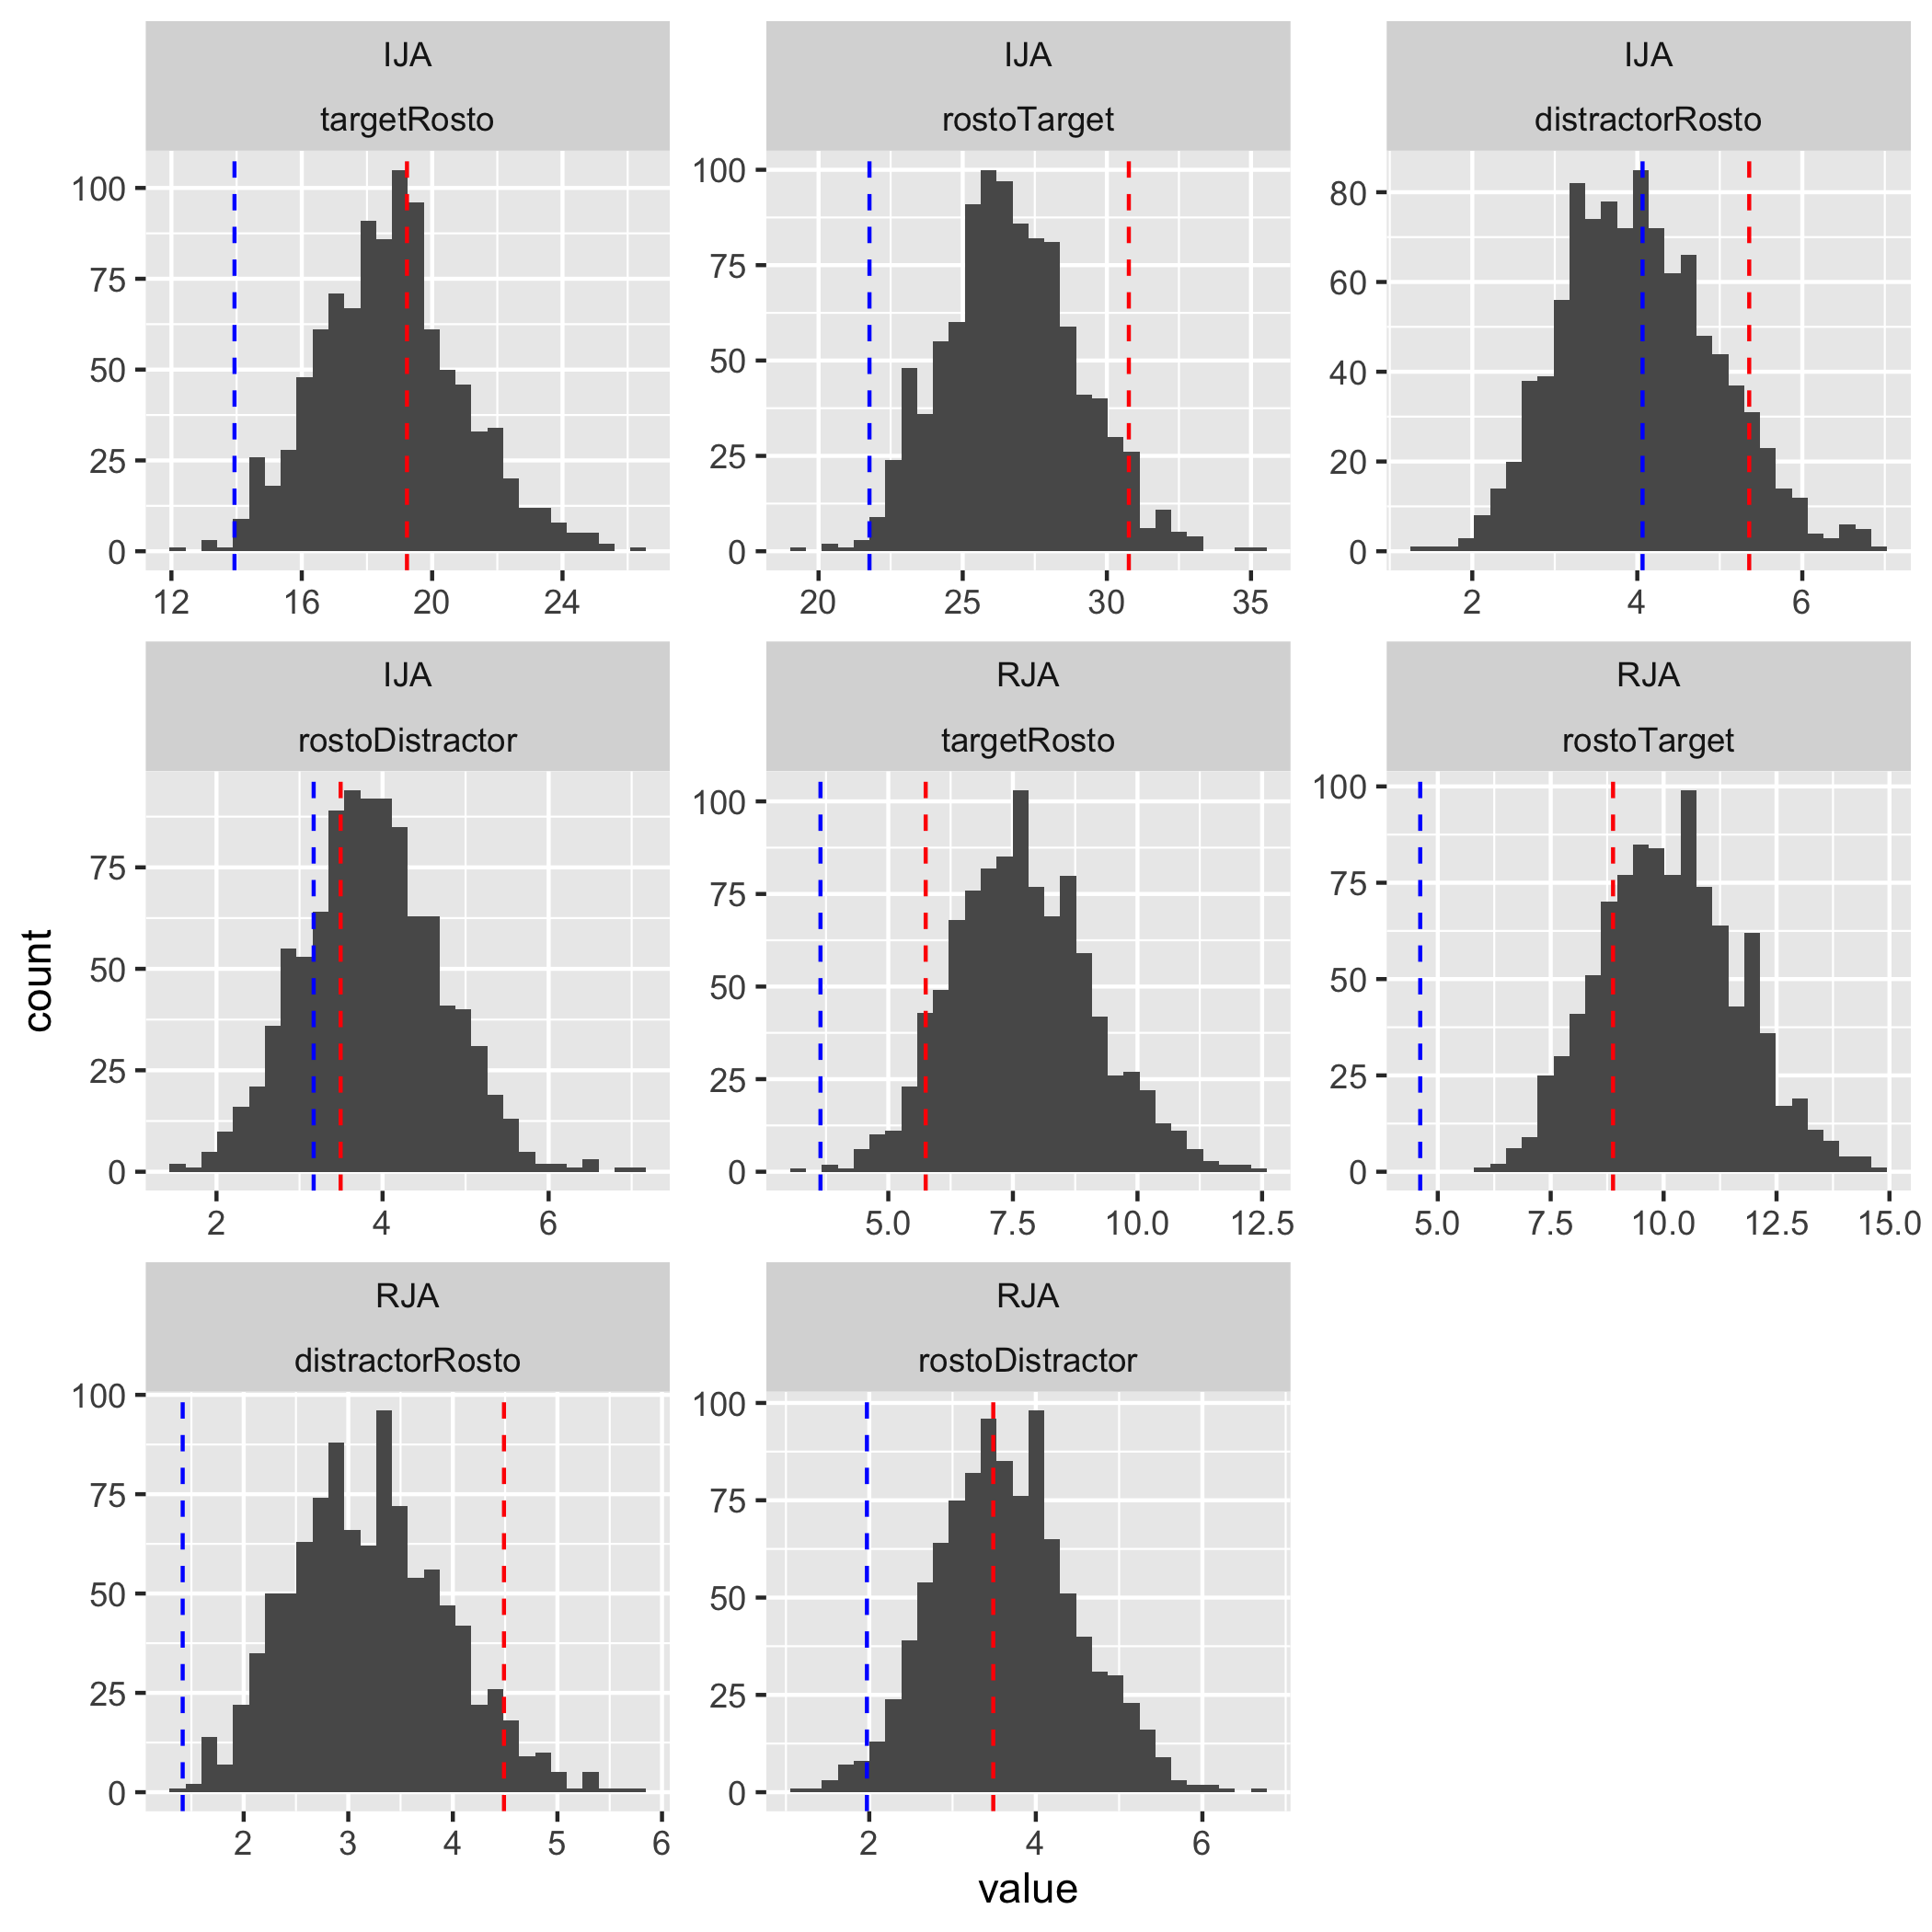
\includegraphics[scale=0.2]{./alternanciasBlueTEA.png}}
  \centering
\end{figure}

\end{document}

